% ----------------------------------------------------------------- %
%             The Speech Signal Processing Toolkit (SPTK)           %
%             developed by SPTK Working Group                       %
%             http://sp-tk.sourceforge.net/                         %
% ----------------------------------------------------------------- %
%                                                                   %
%  Copyright (c) 1984-2007  Tokyo Institute of Technology           %
%                           Interdisciplinary Graduate School of    %
%                           Science and Engineering                 %
%                                                                   %
%                1996-2016  Nagoya Institute of Technology          %
%                           Department of Computer Science          %
%                                                                   %
% All rights reserved.                                              %
%                                                                   %
% Redistribution and use in source and binary forms, with or        %
% without modification, are permitted provided that the following   %
% conditions are met:                                               %
%                                                                   %
% - Redistributions of source code must retain the above copyright  %
%   notice, this list of conditions and the following disclaimer.   %
% - Redistributions in binary form must reproduce the above         %
%   copyright notice, this list of conditions and the following     %
%   disclaimer in the documentation and/or other materials provided %
%   with the distribution.                                          %
% - Neither the name of the SPTK working group nor the names of its %
%   contributors may be used to endorse or promote products derived %
%   from this software without specific prior written permission.   %
%                                                                   %
% THIS SOFTWARE IS PROVIDED BY THE COPYRIGHT HOLDERS AND            %
% CONTRIBUTORS "AS IS" AND ANY EXPRESS OR IMPLIED WARRANTIES,       %
% INCLUDING, BUT NOT LIMITED TO, THE IMPLIED WARRANTIES OF          %
% MERCHANTABILITY AND FITNESS FOR A PARTICULAR PURPOSE ARE          %
% DISCLAIMED. IN NO EVENT SHALL THE COPYRIGHT OWNER OR CONTRIBUTORS %
% BE LIABLE FOR ANY DIRECT, INDIRECT, INCIDENTAL, SPECIAL,          %
% EXEMPLARY, OR CONSEQUENTIAL DAMAGES (INCLUDING, BUT NOT LIMITED   %
% TO, PROCUREMENT OF SUBSTITUTE GOODS OR SERVICES; LOSS OF USE,     %
% DATA, OR PROFITS; OR BUSINESS INTERRUPTION) HOWEVER CAUSED AND ON %
% ANY THEORY OF LIABILITY, WHETHER IN CONTRACT, STRICT LIABILITY,   %
% OR TORT (INCLUDING NEGLIGENCE OR OTHERWISE) ARISING IN ANY WAY    %
% OUT OF THE USE OF THIS SOFTWARE, EVEN IF ADVISED OF THE           %
% POSSIBILITY OF SUCH DAMAGE.                                       %
% ----------------------------------------------------------------- %
\hypertarget{sin}{}
\name{sin}{generate sinusoidal sequence}{signal generation}

\begin{synopsis}
\item[sin] [ --l $L$ ] [ --p $P$ ] [ --m $M$ ]
\end{synopsis}

\begin{qsection}{DESCRIPTION}
{\em sin} generates a discrete sin wave sequence 
of period $P$, length $L$ and magnitude $M$ of the form, 
\begin{displaymath}
  x(n) = M \cdot \sin \left( \frac{2\pi}{P} \cdot n \right), 
\end{displaymath}
and sends the result to standard output.

Both input and output data are in float format.
\end{qsection}

\begin{options}
	\argm{l}{L}{length\\
                        If $L \le 0$, sin values will be
                        generated indefinitely.}{256}
	\argm{p}{P}{period}{10.0}
	\argm{m}{M}{magnitude}{1.0}
\end{options}

\begin{qsection}{EXAMPLE}
In the following example, a sin wave sequence is passed through
a Blackman window and the results are displayed on the screen:
\begin{quote}
\verb!sin -p 12.3 | window | fdrw | xgr!
\end{quote}
\begin{center}
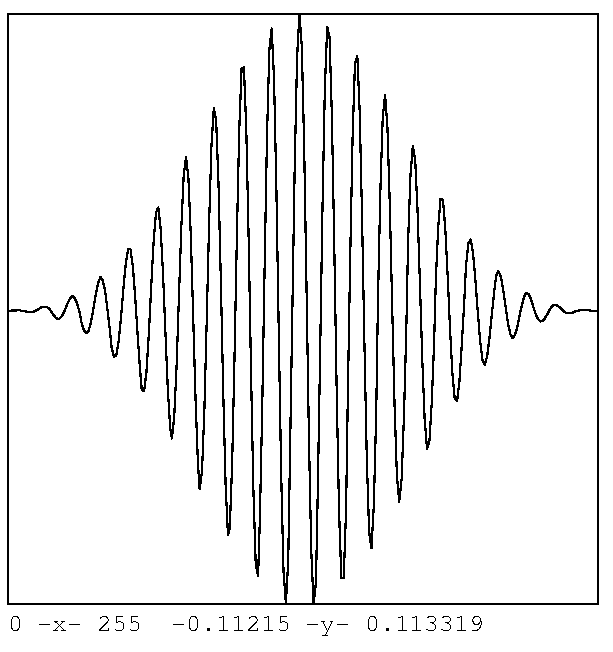
\includegraphics[width=6cm]{fig/sin.pdf}
\end{center}
\end{qsection}

\begin{qsection}{NOTICE}
If $L<0$, generate infinite sequence.
\end{qsection}

\begin{qsection}{SEE ALSO}
\hyperlink{impulse}{impulse},
\hyperlink{step}{step},
\hyperlink{train}{train},
\hyperlink{ramp}{ramp}
\end{qsection}
